% Fichier : sections/03_modele_donnees.tex
\section{Modèle de Données et Structure de Base}

\subsection{Conception du modèle relationnel}

La conception du modèle de données de Running App repose sur une approche relationnelle classique qui privilégie la cohérence, l'intégrité et l'efficacité des requêtes. Cette structure de données constitue le socle de notre application et doit pouvoir évoluer pour accompagner les futures fonctionnalités tout en maintenant les performances du système.

Notre modèle s'organise autour de cinq entités principales qui reflètent les concepts métier fondamentaux de l'application. Chaque entité encapsule un ensemble cohérent d'informations et définit des relations précises avec les autres entités du système. Cette approche nous permet de maintenir la normalisation de la base de données tout en optimisant les accès pour les cas d'usage les plus fréquents.

La table centrale \texttt{users} stocke les informations des utilisateurs et sert de point d'ancrage pour toutes les autres données personnalisées. Cette table contient non seulement les informations d'identification et de profil, mais aussi des métadonnées importantes comme les dates de création et de dernière modification qui facilitent l'audit et la maintenance du système.

Les données de performance sont organisées dans la table \texttt{runs} qui enregistre chaque session de course avec un niveau de détail suffisant pour permettre des analyses ultérieures. Cette table maintient un équilibre entre la richesse des informations stockées et l'efficacité des requêtes, en évitant la sur-normalisation qui pourrait pénaliser les performances.

\begin{infobox}[Principe de conception]
Notre modèle de données équilibre normalisation et performance en regroupant les informations fréquemment consultées ensemble tout en maintenant l'intégrité référentielle entre les entités.
\end{infobox}

\subsection{Description détaillée des entités}

La table \texttt{users} constitue le cœur de notre système d'authentification et de personnalisation. Elle stocke les informations essentielles de chaque utilisateur dans une structure optimisée pour les accès fréquents. Le champ \texttt{password\_hash} utilise un algorithme de hachage sécurisé qui protège les mots de passe même en cas de compromission de la base de données. Le booléen \texttt{is\_admin} permet une gestion simple mais efficace des droits d'administration, tandis que les timestamps de création et de modification facilitent l'audit et la maintenance.

\begin{table}[h]
\centering
\begin{tabular}{|l|l|l|p{5cm}|}
\hline
\textbf{Champ} & \textbf{Type} & \textbf{Contraintes} & \textbf{Description} \\
\hline
id & INT & PRIMARY KEY, AUTO\_INCREMENT & Identifiant unique \\
\hline
username & VARCHAR(50) & UNIQUE, NOT NULL & Nom d'utilisateur unique \\
\hline
email & VARCHAR(100) & UNIQUE, NOT NULL & Adresse email unique \\
\hline
password\_hash & VARCHAR(255) & NOT NULL & Hash sécurisé du mot de passe \\
\hline
first\_name & VARCHAR(50) & NOT NULL & Prénom de l'utilisateur \\
\hline
last\_name & VARCHAR(50) & NOT NULL & Nom de famille \\
\hline
is\_admin & BOOLEAN & DEFAULT FALSE & Indicateur de droits admin \\
\hline
created\_at & TIMESTAMP & DEFAULT CURRENT\_TIMESTAMP & Date de création \\
\hline
updated\_at & TIMESTAMP & DEFAULT CURRENT\_TIMESTAMP & Dernière modification \\
\hline
\end{tabular}
\caption{Structure de la table users}
\end{table}

La table \texttt{runs} capture l'essence de chaque session de course avec un niveau de détail qui permet des analyses sophistiquées tout en restant efficace pour les requêtes courantes. Les champs temporels utilisent le type TIMESTAMP pour une précision à la seconde, suffisante pour les analyses de performance tout en évitant la complexité de types plus précis. La durée stockée en secondes facilite les calculs arithmétiques, tandis que la distance en mètres permet une précision adaptée aux besoins de l'application.

Le champ \texttt{route\_data} mérite une attention particulière car il stocke les coordonnées GPS sous format JSON, permettant une flexibilité maximale pour les analyses géographiques futures. Cette approche hybride, combinant structure relationnelle et flexibilité NoSQL, offre le meilleur des deux mondes pour notre cas d'usage spécifique.

\begin{table}[h]
\centering
\begin{tabular}{|l|l|l|p{4.5cm}|}
\hline
\textbf{Champ} & \textbf{Type} & \textbf{Contraintes} & \textbf{Description} \\
\hline
id & INT & PRIMARY KEY, AUTO\_INCREMENT & Identifiant unique \\
\hline
user\_id & INT & FOREIGN KEY, NOT NULL & Référence vers users.id \\
\hline
start\_time & TIMESTAMP & NOT NULL & Heure de début de course \\
\hline
end\_time & TIMESTAMP & NOT NULL & Heure de fin de course \\
\hline
duration & INT & NOT NULL & Durée en secondes \\
\hline
distance & DECIMAL(8,2) & NOT NULL & Distance en mètres \\
\hline
avg\_speed & DECIMAL(5,2) & NULL & Vitesse moyenne en m/s \\
\hline
max\_speed & DECIMAL(5,2) & NULL & Vitesse maximale en m/s \\
\hline
calories & INT & NULL & Calories brûlées estimées \\
\hline
route\_data & JSON & NULL & Coordonnées GPS du parcours \\
\hline
created\_at & TIMESTAMP & DEFAULT CURRENT\_TIMESTAMP & Date d'enregistrement \\
\hline
\end{tabular}
\caption{Structure de la table runs}
\end{table}

\subsection{Relations et contraintes d'intégrité}

Les relations entre entités sont conçues pour maintenir la cohérence des données tout en optimisant les performances des requêtes les plus fréquentes. La relation principale connecte chaque course à son utilisateur via une clé étrangère qui garantit l'intégrité référentielle.

Cette relation un-à-plusieurs entre \texttt{users} et \texttt{runs} utilise une contrainte \texttt{ON DELETE CASCADE} qui assure la suppression automatique de toutes les courses d'un utilisateur si son compte est supprimé. Cette approche évite les données orphelines tout en simplifiant la maintenance de la base de données.

Les contraintes d'intégrité incluent également des validations au niveau base de données qui complètent les validations applicatives. Par exemple, la durée d'une course ne peut pas être négative, et les timestamps de fin doivent être postérieurs aux timestamps de début. Ces contraintes constituent une couche de sécurité supplémentaire qui protège contre les erreurs de programmation et les tentatives de manipulation malveillante.

\subsection{Diagramme Entité-Relation}

\begin{figure}[h]
\centering
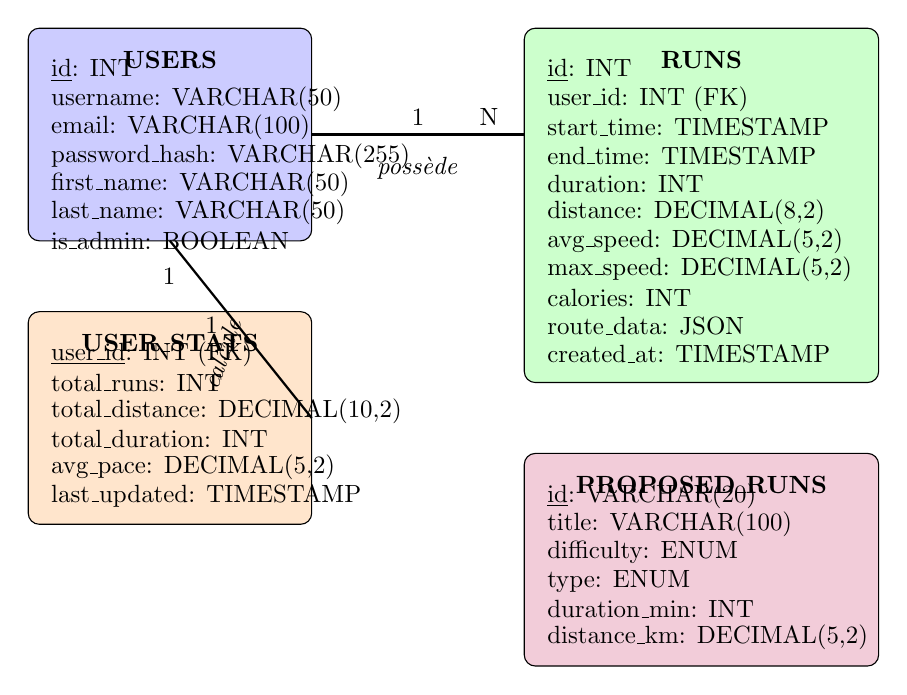
\begin{tikzpicture}[scale=0.9, every node/.style={scale=0.9}]

% Entité Users
\draw[fill=blue!20, rounded corners] (0,6) rectangle (4,9);
\node[anchor=north] at (2,8.8) {\textbf{USERS}};
\node[anchor=west] at (0.2,8.4) {\underline{id}: INT};
\node[anchor=west] at (0.2,8.0) {username: VARCHAR(50)};
\node[anchor=west] at (0.2,7.6) {email: VARCHAR(100)};
\node[anchor=west] at (0.2,7.2) {password\_hash: VARCHAR(255)};
\node[anchor=west] at (0.2,6.8) {first\_name: VARCHAR(50)};
\node[anchor=west] at (0.2,6.4) {last\_name: VARCHAR(50)};
\node[anchor=west] at (0.2,6.0) {is\_admin: BOOLEAN};

% Entité Runs
\draw[fill=green!20, rounded corners] (7,4) rectangle (12,9);
\node[anchor=north] at (9.5,8.8) {\textbf{RUNS}};
\node[anchor=west] at (7.2,8.4) {\underline{id}: INT};
\node[anchor=west] at (7.2,8.0) {user\_id: INT (FK)};
\node[anchor=west] at (7.2,7.6) {start\_time: TIMESTAMP};
\node[anchor=west] at (7.2,7.2) {end\_time: TIMESTAMP};
\node[anchor=west] at (7.2,6.8) {duration: INT};
\node[anchor=west] at (7.2,6.4) {distance: DECIMAL(8,2)};
\node[anchor=west] at (7.2,6.0) {avg\_speed: DECIMAL(5,2)};
\node[anchor=west] at (7.2,5.6) {max\_speed: DECIMAL(5,2)};
\node[anchor=west] at (7.2,5.2) {calories: INT};
\node[anchor=west] at (7.2,4.8) {route\_data: JSON};
\node[anchor=west] at (7.2,4.4) {created\_at: TIMESTAMP};

% Entité User Statistics (calculées)
\draw[fill=orange!20, rounded corners] (0,2) rectangle (4,5);
\node[anchor=north] at (2,4.8) {\textbf{USER\_STATS}};
\node[anchor=west] at (0.2,4.4) {\underline{user\_id}: INT (FK)};
\node[anchor=west] at (0.2,4.0) {total\_runs: INT};
\node[anchor=west] at (0.2,3.6) {total\_distance: DECIMAL(10,2)};
\node[anchor=west] at (0.2,3.2) {total\_duration: INT};
\node[anchor=west] at (0.2,2.8) {avg\_pace: DECIMAL(5,2)};
\node[anchor=west] at (0.2,2.4) {last\_updated: TIMESTAMP};

% Entité Proposed Runs
\draw[fill=purple!20, rounded corners] (7,0) rectangle (12,3);
\node[anchor=north] at (9.5,2.8) {\textbf{PROPOSED\_RUNS}};
\node[anchor=west] at (7.2,2.4) {\underline{id}: VARCHAR(20)};
\node[anchor=west] at (7.2,2.0) {title: VARCHAR(100)};
\node[anchor=west] at (7.2,1.6) {difficulty: ENUM};
\node[anchor=west] at (7.2,1.2) {type: ENUM};
\node[anchor=west] at (7.2,0.8) {duration\_min: INT};
\node[anchor=west] at (7.2,0.4) {distance\_km: DECIMAL(5,2)};

% Relations
\draw[thick] (4,7.5) -- (7,7.5);
\node[above] at (5.5,7.5) {1};
\node[above] at (6.5,7.5) {N};
\node[below] at (5.5,7.3) {\textit{possède}};

\draw[thick] (4,3.5) -- (2,6);
\node[left] at (2.8,4.8) {1};
\node[left] at (2.2,5.5) {1};
\node[below, rotate=70] at (2.5,4.5) {\textit{calcule}};

\end{tikzpicture}
\caption{Diagramme Entité-Relation de Running App}
\end{figure}

\subsection{Optimisations et indexation}

L'optimisation de la base de données constitue un aspect crucial pour maintenir des performances acceptables même avec une large base d'utilisateurs. Notre stratégie d'indexation cible les requêtes les plus fréquentes identifiées lors de l'analyse des cas d'usage.

L'index principal sur \texttt{runs(user\_id, start\_time)} optimise les requêtes d'historique personnel, qui représentent la majorité des accès à cette table. Cet index composite permet de récupérer efficacement toutes les courses d'un utilisateur triées par date, ce qui correspond au cas d'usage le plus courant de consultation du tableau de bord personnel.

Un second index sur \texttt{runs(start\_time)} facilite les requêtes statistiques globales et les analyses temporelles qui peuvent être nécessaires pour les fonctionnalités d'administration ou les rapports de performance du système. Cet index permet également d'optimiser les requêtes de recherche par période sans spécifier d'utilisateur particulier.

La table \texttt{users} bénéficie d'index uniques sur les champs \texttt{email} et \texttt{username}, non seulement pour garantir l'unicité mais aussi pour accélérer les requêtes d'authentification qui constituent un point critique pour l'expérience utilisateur.

\begin{successbox}[Stratégie d'optimisation]
\begin{itemize}[leftmargin=1cm]
\item Index composites sur les colonnes fréquemment utilisées ensemble
\item Partitionnement temporel envisagé pour les données historiques
\item Dénormalisation sélective pour les statistiques couramment consultées
\item Mise en cache applicative pour les données statiques
\end{itemize}
\end{successbox}

\subsection{Évolution et migration du schéma}

La gestion des évolutions du schéma de base de données constitue un défi important dans le cycle de vie d'une application. Notre approche utilise Flask-Migrate qui s'appuie sur Alembic pour gérer les migrations de manière versionnée et reproductible.

Chaque modification du modèle de données génère un script de migration qui peut être appliqué de manière incrémentale sur les environnements de développement, de test et de production. Cette approche garantit que tous les environnements restent synchronisés et que les déploiements peuvent être effectués en toute sécurité.

Les migrations incluent non seulement les modifications de structure mais aussi les transformations de données nécessaires lors de changements de format ou de contraintes. Par exemple, l'ajout d'une nouvelle colonne obligatoire s'accompagne automatiquement de la logique pour populer cette colonne avec des valeurs par défaut appropriées pour les enregistrements existants.

Notre stratégie de migration privilégie les changements rétrocompatibles autant que possible, en utilisant des techniques comme l'ajout de colonnes optionnelles suivi d'une phase de transition avant de rendre ces colonnes obligatoires. Cette approche minimise les risques lors des déploiements et permet des rollbacks en cas de problème.

\subsection{Sauvegarde et récupération}

La stratégie de sauvegarde protège contre la perte de données tout en maintenant des performances acceptables pour les opérations courantes. Notre approche combine sauvegardes complètes périodiques et sauvegardes incrémentales plus fréquentes pour optimiser l'espace de stockage et les temps de récupération.

Les sauvegardes complètes sont programmées quotidiennement pendant les heures de faible activité, tandis que les sauvegardes incrémentales capturent les modifications toutes les heures. Cette stratégie permet de restaurer le système avec une perte de données maximale d'une heure, ce qui constitue un compromis acceptable pour notre cas d'usage.

Les scripts de sauvegarde incluent des vérifications d'intégrité qui détectent automatiquement les corruptions potentielles et déclenchent des alertes en cas de problème. Ces vérifications portent sur la cohérence des contraintes d'intégrité, la validité des formats de données et la complétude des sauvegardes.

La procédure de récupération est documentée et testée régulièrement pour garantir qu'elle peut être exécutée rapidement en cas d'incident. Les tests de récupération incluent la restauration sur un environnement de test et la vérification que toutes les fonctionnalités de l'application restent opérationnelles après restauration.